\documentclass[twoside,a5paper]{memoir}

\usepackage[utf8]{inputenc}
\usepackage[english]{babel}
\usepackage{biblatex}
\addbibresource{references.bib}

\usepackage{amsmath}
\usepackage{hyperref}
\usepackage{fontspec}
\usepackage{unicode-math}
\usepackage{graphicx}
\usepackage[super]{nth}
\usepackage{booktabs}
\usepackage{geometry}
\usepackage{csquotes}
\usepackage{multirow}
\usepackage{cleveref}
%\usepackage[Glenn]{fncychap}
\usepackage{tikz}

\nonfrenchspacing

\begin{document}

\setmathfont{STIXTwoMath}[
  Extension={.otf},
  Path={./fonts/},
  Scale=1]

\setmainfont{STIXTwoText}[
  Extension={.otf},
  Path={./fonts/},
  UprightFont={*-Regular},
  BoldFont={*-Bold},
  ItalicFont={*-Italic},
  BoldItalicFont={*-BoldItalic}]

\title{\scshape Data science \\ \large Foundations and practices}
\author{Filipe A. N. Verri}

\maketitle

\tableofcontents

\chapter{Preface}

\noindent Dear reader, \vspace{1em}

This book is based on the lecture notes from my course PO-235 Data Science Project, which
I teach to graduate students at both the Aeronautics Institute of Technology (ITA) and the
Federal University of São Paulo (UNIFESP) in Brazil.  I have been teaching this subject
since 2021, and I have continually updated the material each year.

Also, I was the coordinator of the Data Science Specialization Program (CEDS) at ITA.
That experience, which included a great deal of administrative work, as well as teaching and
supervising professionals in the course, has helped me to understand the needs of the
market and the students.

Moreover, parts of the project development methodology presented here came from my
experience as a lead data scientist in R\&D projects for the Brazilian Air Force,
which included projects in areas such as image processing, natural language processing,
and spatio-temporal data analysis.

Literature provides us with a wide range of excellent theoretical material on machine learning and
statistics, and highly regarded practical books on data science tools.  However, I missed
something that could provide a solid foundation on data science, covering all steps in a
data science project, including its software engineering aspects.

My goal is to provide a book that serves as a textbook for a course on data science
projects or as a reference for professionals working in the field.  I strive to maintain a
formal tone while preserving the practical aspects of the subject.  I do not focus on
a specific tool or programming language, but rather seek to explain the semantics of data
science tasks that can be implemented in any programming language.

Also, instead of teaching specific machine learning algorithms, I try to explain why
machine learning works, thereby increasing awareness of its pitfalls and limitations.
For this purpose, I assume you have a strong mathematical and statistical foundation.

One important artificial constraint I have imposed in the material (for the sake of the
course) is that I only consider predictive methods, more specifically inductive ones. I do
not address topics such as clustering, association rule mining, transductive learning,
anomaly detection, time series forecasting, reinforcement learning, etc.

I expect my approach on the subject to provide understanding of all steps in a data
science project, including a deeper focus on correct evaluation and validation of data
science solutions.

Note that, in this book, I openly express my opinions and beliefs. On several occasions it
may sound controversial.  I am not trying to be rude or to demean any researcher or
practitioner in the field; rather, I aim to be honest and transparent.

\vspace{1em}
\emph{I'd rather be bold and straightforward than cower about my beliefs.}
\vspace{1em}

I hope you enjoy reading.

\section*{Contributors}

I would like to thank the following contributors for their help in improving this book:

\begin{itemize}
  \itemsep0em
  \item Johnny C. Marques
  \item Manoel V. Machado (aka \emph{ryukinix})
  \item Vitor V. Curtis
\end{itemize}

All contributors have freely waived their rights to the content they contributed to this book.

% vim: set spell spelllang=en:

\chapter{Course plan}

In the following, I present the course plan for PO-235 and CMC-16.

Any questions about the classes should be sent via Google Classroom.  If your question is
of general interest, please use the main stream.  If your question is personal and about
a specific assignment or grade, please use the private stream.

\newpage
\thispagestyle{empty}
\section*{PO-235 Data science project}

\emph{Course plan (\the\year{})}

Prof. Filipe A. N. Verri

\paragraph{Important:} Only graduate students are allowed to take this course.

\paragraph{Number of students:} Approx. 20

\paragraph{Course load:} 3--0--0--4

\paragraph{Requirements:} Advanced programming skills, strong statistics background, and
beginner level machine learning skills.

\paragraph{Course program:}
Brief history of data science.  Fundamental data concepts. Stages in a Data Science
project.  Data Infrastructure. Data integration from multiple sources. Data engineering
and shaping.  Inductive learning and principles of statistical learning theory.
Application of machine learning models in real-world problems.  Experimental planning for
data science. Model evaluation and Bayesian analysis.  Documentation and deployment.
Ethical and legal issues in data science.  Privacy-preserving computational approaches.

\paragraph{Goals:}
Providing the theoretical background and the practical concepts to develop an end-to-end
data science project for an inductive task.

\paragraph{Teaching methodology:}
Expository classes in common classroom, using whiteboard, slide presentations, coding
examples, books and scientific papers. Supplementary didactic materials will be available
in Google Classroom. The development of the case study will happen during home study
hours, including programming and scientific paper writing.  All classes will be given in
English.  Students are encouraged to ask questions in English, but Portuguese is also
allowed. All written and oral assignments must be in English.

\paragraph{Grading:} Two individual written tests in the \nth{1} ($T_1$ and $T_2$) and
another in the \nth{2} quarter ($T_3$).  Also, a group activity that includes writting a
scientific paper, developing a data science product, and a 30 minutes presentation ($L$).

Final grades will be calculated as
\begin{equation*}
  \text{\nth{1} Q} = \sqrt{T_1 T_2}\text{,} \qquad
  \text{\nth{2} Q} = \sqrt{T_3 L}\text{,} \qquad
  \text{Exam} = L\text{.}
\end{equation*}

\paragraph{Case study:} Exactly 6 groups will be formed.  Each group will be responsible for
a case study.  Students must choose a real-world problem and develop a data science
project, including data collection, data transformation, inductive learning, validation,
documentation, and deployment.  The results must be presented in a scientific paper
format and a 30 minutes presentation.  The trained models must be incorporated in a
data science product, such as a web application, a mobile application, or a web service.

\paragraph{Bibliography:}
\begin{itemize}
  \itemsep 0pt
  \item \fullcite{Zumel2019}.
  \item \fullcite{Wickham2023}.
  \item \fullcite{Kelleher2018}.
\end{itemize}

The first two books (\citeauthor{Zumel2019,Wickham2023}) are available online for free.

% \paragraph{Must read:}
% \begin{itemize}
%   \itemsep 0pt
%   \item In-progress textbook at \href{https://comp.ita.br/~verri/dsp-book}{comp.ita.br/~verri/dsp-book}.
%   \item \fullcite{Vapnik1999}.
%   \item \fullcite{Benavoli2017}.
% \end{itemize}

Any required extra material will be made available in Google Classroom.
\thispagestyle{empty}

\newpage
\paragraph{Calendar:} The expected schedule is presented below.
\thispagestyle{empty}

\begin{center}
  \begin{tabular}{ll}
    \toprule
    \multicolumn{2}{c}{\bfseries \nth{1} Quarter} \\
    \midrule
    Week & Topics \\
    \midrule
    \multirow{2}{*}{1} & Brief history of data science \pcref{chap:history} \\
      & Preliminaries \pcref{chap:preliminaries} \\
    \midrule
    2 & \bfseries Written test \\
    \midrule
    \multirow{2}{*}{3} & Fundamental data concepts \pcref{chap:data} \\
      & Stages in a data science project \\
    \midrule
    4 & \multirow{2}{*}{Inductive learning and statistical learning theory} \\
    5 &  \\
    \midrule
    6 & Data infrastructure and data integration from multiple sources \\
    \midrule
    7 & Data engineering and shaping \\
    \midrule
    8 & \bfseries Written test \\
    \bottomrule
  \end{tabular}
\end{center}

\begin{center}
  \begin{tabular}{ll}
    \toprule
    \multicolumn{2}{c}{\bfseries \nth{2} Quarter} \\
    \midrule
    Week & Topics \\
    \midrule
    1 & \multirow{2}{*}{Application of machine learning models in real-world problems} \\
    2 &  \\
    \midrule
    3 & \multirow{2}{*}{Experimental planning for data science} \\
    4 & \\
    \midrule
    5 & \multirow{2}{*}{Model evaluation and Bayesian analysis} \\
    6 & \\
    \midrule
    7 & \bfseries Written test \\
    \midrule
    \multirow{3}{*}{8} & Documentation and deployment \\
      & Ethical and legal issues in data science \\
      & Privacy-preserving computational approaches \\
    \bottomrule
  \end{tabular}
\end{center}

Case studies will be presented during exam weeks.  At most 3 case studies will be
presented per day, with 30 minutes for each presentation and 20 minutes for questions.

\thispagestyle{empty}

\newpage
\thispagestyle{empty}
\section*{CMC-16 Data science practices}

\emph{Course plan (\the\year{})}

Prof. Filipe A. N. Verri

\paragraph{Important:} Only ITA's undergraduate students are allowed to take this course.

\paragraph{Number of students:} Approx. 20 (no more than 40 students)

\paragraph{Course load:} 2--0--1--5

\paragraph{Requirements:} CMC-13 or CMC-15

\paragraph{Course program:}
Brief history of Data Science. Stages in a Data Science project. Tidy Data. Data
integration from multiple sources. Data engineering and shaping. Inductive learning and
statistical learning theory. Experimental planning for Data Science. Model evaluation and
Bayesian Analysis. Documentation and deployment. Privacy-preserving computational
approaches.

\paragraph{Goals:}
Further studying the practical aspects of Data Science (in relation to CMC-13) and providing
the mathematical foundations to ensure the correct usage of Data Science techniques.

The specific goals are:
\begin{itemize}
  \item Understanding the steps and people involved in Data Science projects;
  \item Developing an end-to-end case study, including data collection, data transformation,
    inductive learning, validation, documentation, and deployment; and
  \item Critically evaluate the results and implications of the case study.
\end{itemize}

\paragraph{Teaching methodology:}
Expository classes in common classroom, using whiteboard, slide presentations, coding
examples, books and scientific papers. Supplementary didactic materials will be available
in Google Classroom. The development of the case study will happen during laboratory
classes and home study hours, including programming and writing essays.

\paragraph{Grading:} One individual written test in the \nth{1} and another in the \nth{2} quarter.
Essay and oral presentation about the case study (in groups) for the final exam.

\paragraph{Case study:} Exactly 6 groups will be formed.  Each group will be responsible for
a case study.  Students must choose a real-world problem and develop a data science
project, including data collection, data transformation, inductive learning, validation,
documentation, and deployment.  The results must be presented in a short essay (max. 3
pages) and a 30 minutes presentation.  The trained models must be incorporated in a data
science product, such as a web application, a mobile application, or a web service.

\thispagestyle{empty}
\paragraph{Bibliography:}
\begin{itemize}
  \item Nina Zumel and John Mount. Practical Data Science with R. Manning, 2nd Edition, 2019.
  \item Hadley Wickham and Garret Grolemund, R for Data Science: Import, Tidy, Transform, Visualize, and Model Data. O’Reilly Media, 2017.
  \item John D. Kelleher and Brendan Tierney. Data Science, MIT Press, 2018.
\end{itemize}

The first two books (Zumel and Mount, and Wickham and Grolemund) are available online for free.

\thispagestyle{empty}
\paragraph{Recommended reading:}
\begin{itemize}
  \item In-progress textbook at \href{https://comp.ita.br/~verri/dsp-book}{comp.ita.br/\textasciitilde{}verri/dsp-book}.
  \item \fullcite{Vapnik1999}.
  \item \fullcite{Benavoli2017}.
\end{itemize}
Any extra material will be made available in Google Classroom.

\newpage
\paragraph{Calendar:} The expected schedule is presented below.
\thispagestyle{empty}

\begin{center}
  \begin{tabular}{ll}
    \toprule
    \multicolumn{2}{c}{\bfseries \nth{1} Quarter} \\
    \midrule
    Week & Topics \\
    \midrule
    1 & Brief history of Data Science and CMC-13 review \\
    2 & Stages in a Data Science project \\
    3 & Tidy Data and data integration from multiple sources \\
    4 & Data engineering and shaping \\
    5 & \multirow{2}{*}{Inductive learning and statistical learning theory} \\
    6 &  \\
    7 & Case study discussion and definitions \\
    8 & \bfseries Written test \\
    \bottomrule
  \end{tabular}
\end{center}

\begin{center}
  \begin{tabular}{ll}
    \toprule
    \multicolumn{2}{c}{\bfseries \nth{2} Quarter} \\
    \midrule
    Week & Topics \\
    \midrule
    1 & Experimental planning for Data Science \\
    2 & Model evaluation \\
    3 & Bayesian Analysis \\
    4 & Documentation and deployment \\
    5 & Privacy-preserving computational approaches \\
    6 & \bfseries Written test \\
    7 & \multirow{2}{*}{\bfseries Presentations and discussions} \\
    8 & \\
    \bottomrule
  \end{tabular}
\end{center}

\thispagestyle{empty}

\chapter{Brief history of data science}
\label{chap:history}

\chapterprecishere{``Begin at the beginning,'' the King said gravely, ``and
go on till you come to the end: then stop.''\par\raggedleft--- \textup{Lewis
Carroll}, Alice in Wonderland}

There are many points-of-view about the beginning of data science.  For the sake of
contextualization, I separate the topic in two approaches: the history of the term itself
and a broad timeline of data-driven sciences highlighting the important figures in each
age.

\begin{mainbox}{Chapter remarks}
  \boxsubtitle{Context}

  \begin{itemize}
    \item The term ``data science'' is recent and has been used to label rather different fields.
    \item The history of data-driven sciences is long and rich.
  \end{itemize}

  \boxsubtitle{Objectives}

  \begin{itemize}
    \item Understand the history of the term ``data science.''
    \item Understand the history of data-driven sciences.
  \end{itemize}

  \boxsubtitle{Takeways}

  \begin{itemize}
    \item There is no consensus on the definition of data science.
    \item There is enough evidence to support data science as a new science.
  \end{itemize}
\end{mainbox}

\section{The term ``data science''}

The term data science is recent and has been used to label rather different fields of
study.  In the following, I emphasize the history of a few notable usage of the term.

\def\naurds{(0,0) circle (20mm)}
\def\naurcs{(0:5mm) circle (15mm)}
\def\naurde{(0:40mm) circle (15mm)}

\colorlet{circle edge}{black!50}
\colorlet{circle area}{black!20}

\tikzset{filled/.style={fill=circle area, draw=circle edge, thick},
    outline/.style={draw=circle edge, thick}}

\begin{figure}
  \centering
  \begin{tikzpicture}
    \begin{scope}
      \clip \naurds;
      \fill[filled] \naurcs;
    \end{scope}
    \draw[outline] \naurds node(ds) {};
    \draw[outline] \naurcs node {computer science};
    \draw[outline] \naurde node {domain expertise};
    \node[anchor=north,above] at (0,2) {data science};
  \end{tikzpicture}
  \caption{
    Naur's view of data science.  For him, data science studies the techniques to deal
    with data, but he delegates the meaning of data to other fields.
  }
  \label{fig:naur}
\end{figure}

\paragraph{Peter Naur (1928 -- 2016)}

The term ``data science'' itself was coined in the 1960s by Peter Naur (/naʊə/). Naur was
a Danish computer scientist and mathematician who made significant contributions to the
field of computer science, including his work on the development of programming
languages\footnote{He is best remembered as a contributor, with John Backus, to the
Backus–Naur form (BNF) notation used in describing the syntax for most programming
languages.}.
His ideas and concepts laid the groundwork for the way we think about programming and data
processing today.

\begin{mainbox}{Peter Naur}
  \begin{itemize}
    \item Danish computer scientist and mathematician.
    \item Coined the term ``data science'' in the 1960s.
    \item Proposed the term ``datalogy'' as an alternative to computer science.
  \end{itemize}
\end{mainbox}

Naur disliked the term computer science and suggested it be called datalogy or data
science.  In the 1960s, the subject was practised in Denmark under Peter
Naur's term datalogy, which means the science of data and data processes.

He coined this term to emphasize the importance of data as a fundamental component of
computer science and to encourage a broader perspective on the field that included
data-related aspects. At that time, the field was primarily centered on programming
techniques, but Naur's concept broadened the scope to recognize the intrinsic role of data
in computation.

In his book\footnote{Peter Naur: Concise Survey of Computer Methods, 397 p.
Studentlitteratur, Lund, Sweden, ISBN 91-44-07881-1, 1974.
\url{http://www.naur.com/Conc.Surv.html}}, ``Concise Survey of Computer Methods'', he
parts from the concept that \emph{data} is ``a representation of facts or ideas in a
formalised manner capable of being communicated or manipulated by some
process.''\footnote{I. H. Gould (ed.): ‘IFIP guide to concepts and terms in data
processing’, North-Holland Publ. Co., Amsterdam, 1971.} Note however that his view of the
science only ``deals with data [\dots] while the relation of data to what they represent
is delegated to other fields and sciences.''

\def\clevelandds{(0,0) circle (20mm)}
\def\clevelandst{(0:-5mm) circle (15mm)}
\def\clevelandde {(2,1) circle (15mm)}
\def\clevelandcs {(2,-1) circle (15mm)}

\begin{figure}
  \centering
  \begin{tikzpicture}
    \begin{scope}
      \clip \clevelandds;
      \fill[filled] \clevelandst;
      \fill[filled] \clevelandde;
      \fill[filled] \clevelandcs;
    \end{scope}
    \draw[outline] \clevelandds node(ds) {};
    \draw[outline] \clevelandst node {statistics};
    \draw[outline] \clevelandde node {domain expertise};
    \draw[outline] \clevelandcs node {computer science};
    \node[anchor=north,above] at (0,2) {data science};
  \end{tikzpicture}
  \caption{
    Cleveland's view of data science.  For him, data science is the ``modern'' statistics,
    where it is enlarged by computer science and domain expertise.
  }
  \label{fig:cleveland}
\end{figure}

\paragraph{William Cleveland (born 1943)}

In 2001, a prominent statistician used the term ``data science" in his work to describe a
new discipline that comes from his ``plan to enlarge the major areas of technical work of
the field of statistics\footnote{W. S. Cleveland. Data Science: An Action Plan for
Expanding the Technical Areas of the Field of Statistics. ISI Review, 69:21–26, 2001.}.''
In 2014, that work was republished\footnote{W. S. Cleveland.
Data Science: An Action Plan for the Field of Statistics. Statistical Analysis and Data
Mining, 7:414–417, 2014. reprinting of 2001 article in ISI Review, Vol 69.}.
He advocates the expansion of statistics beyond theory into technical areas, significantly
changing statistics.  Thus, it warranted a new name.

\begin{mainbox}{William Cleveland}
  \begin{itemize}
    \item American statistician.
    \item Proposed the discipline ``data science'' in 2001.
    \item Proposed the term ``data science'' as the new name for expansion of statistics.
  \end{itemize}
\end{mainbox}

As a result, William Swain Cleveland II is credited to define data science as it is most
used today. He is a highly influential figure in the fields of statistics, machine
learning, data visualization, data analysis for multidisciplinary studies, and high
performance computing for deep data analysis.

\paragraph{Buzzword or a new science?}

Be aware that literature has no consensus on the definition of data science, and it is still considered
by some to be a buzzword\footnote{Press, Gil. "Data Science: What's The Half-Life of a
Buzzword?". Forbes. Available at
\url{https://www.forbes.com/sites/gilpress/2013/08/19/data-science-whats-the-half-life-of-a-buzzword/}}.

Most of the usages of the term in literature and in the media are either a rough
reference to a set of data-driven techniques or a marketing strategy.  Naur
(\cref{fig:naur}) and Cleveland (\cref{fig:cleveland}) are among the few that try to
carefully define the term.  However, both of them do not see data science as an
independent field of study, but an enlarged scope of an existing science.  I disagree;
the social and economical demand for data-driven solutions led to an evolution in our
understanding of the challenges we are facing.  As a result, we see many ``data
scientist'' being hired and many ``data science degrees'' programs emerging.

In \cref{chap:data}, I dare to provide a (yet another) definition for the term.  I
argue that its object of study can be precisely established to support it as a new
science.

\begin{mainbox}{A new science}
  \begin{itemize}
    \item Both Naur and Cleveland do not see data science as an independent field of study.
    \item I argue that data science is not a buzzword.
    \item Our social and economical reality demands a new science.
  \end{itemize}
\end{mainbox}

\section{Timeline and historical markers}

\textcite{Kelleher2018} provides an interesting time line of data-driven methods and
influential figures in the field.  I reproduce it here with some minor changes, including
some omissions and additions.

Like \citeauthor{Kelleher2018}, I address data collection, and then data analysis.

\subsection{Timeline of data collection}

The importance of collecting data goes without saying.  Data fuels analysis and
decision making.  In the following, I present some of the most important milestones in the history
of data collection.

% A TikZ picture with the data collection timeline.
\begin{figure}
  \centering
  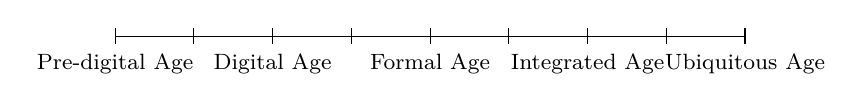
\begin{tikzpicture}
    \draw (0,0) -- (8,0);
    \foreach \x in {0,1,...,8} {
      \draw (\x,-0.1) -- (\x,0.1);
    }
    \foreach \x/\y in {0/Pre-digital Age, 2/Digital Age, 4/Formal Age, 6/Integrated Age, 8/Ubiquitous Age} {
      \node[anchor=north] at (\x,-0.1) {\footnotesize\y};
    }
  \end{tikzpicture}
  \caption{
    Timeline of the ages of data collection.
  }
  \label{fig:collection-history}
\end{figure}

\Cref{fig:collection-history} illutrates the timeline.

\subsubsection{Pre-digital age}

We can consider the earliest records of data collection to be the notches on sticks and
bones to keep tracking of passing of time.  The Lebombo bone, a baboon fibula with
notches, is probably the earliest known mathematical object.  It was found in the Lebombo
Mountains located between South Africa and Eswatini.
They estimate it is more
than 40,000 years old. It is conjectured to be a tally stick, but its exact purpose is
unknown. Its 29 notches suggests that may have been used as a lunar phase counter.
However, since it is broken at one end, the 29 notches may or may not be the total
number\footcite{Beaumont2013}.

Since the early forms of writing, humanity abilities to record events and information
increased significantly.  The first known written records date back to 3,500 BC, the
Sumerian archaic (pre-cuneiform) writing.  This writing system was used to represent
commodities using clay tokens and to record transactions\footcite{Ifrah1998}.

Another important milestone in the history of data collection is the record of
demographic data.  One of first known census was conducted in 3,800 BC in the Babylonian
Empire.  It was ordered to assess the population and resources of
his empire\footcite{Grajalez2013}.

Moving forward many years, I consider a major influential figure in the history of data
collection to be Florence Nightingale (1820 -- 1910).  She was a passionate statistician
and probably the first person to use statistics to influence public and official
opinion.  The meticulous records she kept during the Crimean War
(1853 -- 1856) were the evidence that saved lives.  She was also the first to use
statistical graphics to present data in a way that was easy to understand.  She is
credited with developing a form of the pie chart now known as the polar area
diagram.  She also reformed healthcare in the United Kingdom and
is considered the founder of modern nursing\footcite{Grajalez2013}.

\begin{mainbox}{Florence Nightingale}
  \begin{itemize}
    \item Passionate statistician.
    \item First person to use statistics to influence public and official opinion.
    \item Organized data from garden fruits and vegetables into numerical tables at the age of 9.
    \item At 20 she was receiving two-hour lessons from a Cambridge-trained mathematician.
    \item She found the sight of a long column of figures “perfectly reviving”.
    \item She went out to the Crimean War, to Scutari in Turkey, in 1854.
    \item She found that not even the numbers of soldiers entering the hospitals, or leaving them – alive or dead – was known.
    \item From the first she kept meticulous records.
    \item The data she collected was the evidence that saved lives.
    \item She was the first to use statistical graphics to present data in a way that was easy to understand.
    \item She is credited with developing a form of the pie chart now known as the polar area diagram.
    \item She reformed healthcare in the United Kingdom and is considered the founder of modern nursing.
  \end{itemize}
\end{mainbox}

\subsection{Timeline of data analysis}

\begin{itemize}
  \item Summary statistics
  \item Probability Advent 17, 18th
  \item Statistical learning 19th
    \begin{itemize}
      \item Bayes rule
      \item Gauss’ method of least squares
      \item Playfair data visualization
    \end{itemize}
  \item 20th inference
    \begin{itemize}
      \item Pearson hypothesis testing
      \item Fisher multivariate analysis, maximum likelihood estimate
    \end{itemize}
  \item Computer: McCulloch Pitts, Shannon information theory, Fix and Hodged discriminatory analysis, knn
  \item Machine learning: 1965 Nils Nilsson neural network, 1966 Hunt inducing trees, Kmeans, Vapnik 71
  \item Today: Ensembles, Deep learning: vision and language, KDD
\end{itemize}

\chapter{Preliminaries}
\label{chap:preliminaries}

\chapterprecishere{%
  Maar ik maak steeds wat ik nog niet kan om het te leeren kunnen.\par\raggedleft---
  \textup{Vincent van Gogh}, The Complete Letters of Vincent Van Gogh, Volume Three}

Foundamental concepts in data science come from a variety of fields, including
mathematics, statistics, computer science, optimization theory, and information theory.
This chapter provides a brief overview of the computational, mathematical and statistical
concepts that are used in the rest of the book.

\section{Algorithms and data structures}

Algorithms are step-by-step procedures for solving a problem.  They are used to
manipulate data structures, which are ways of organizing data to solve problems.
They are realized in programming languages, which are formal languages that can be used
to express algorithms.

\subsection{Algoritmic paradigms}

Some techniques are used to solve a wide variety of problems.  They are called
algorithmic paradigms.  The most common ones are listed below.

\paragraph{Divide and conquer}  The problem is divided into smaller subproblems that are
solved recursively.  The solutions to the subproblems are then combined to give a solution
to the original problem.

\paragraph{Dynamic programming}  The problem is divided into overlapping subproblems, and
the solutions to the subproblems are only solved once. The subproblems are then optimized
to find the overall solution.

\paragraph{Greedy algorithms}  The problem is solved with incremental steps, each of which
is locally optimal.  The overall solution is not guaranteed to be optimal.

\subsection{Computational complexity}

Big-O notation, time and space complexity, NP-completeness.

\subsection{Data structures}

Arrays, linked lists, stacks, queues, trees, graphs, hash tables.

\section{Linear algebra}

\subsection{Vectors and matrices}

\subsection{Matrix decompositions}

\textcolor{red}{Verify!}

\paragraph{Singular value decomposition} The singular value decomposition (SVD) of a
matrix $A$ is a factorization of the form
\begin{equation}
  \label{eq:svd}
  A = U \Sigma V^T\text{,}
\end{equation}
where $U$ and $V$ are orthogonal matrices and $\Sigma$ is a diagonal
matrix with non-negative real numbers on the diagonal.  The singular values are the
diagonal entries of $\Sigma$.

\paragraph{Eigenvalue decomposition}  The eigenvalue decomposition of a matrix $A$
is a factorization of the form
\begin{equation}
  \label{eq:eigdec}
  A = Q \Lambda Q^{-1}\text{,}
\end{equation}
where $Q$ is a square matrix whose columns are the eigenvectors of $A$, and
$\Lambda$ is a diagonal matrix whose diagonal entries are the eigenvalues of
$A$.

\paragraph{Cholesky decomposition}  The Cholesky decomposition of a positive-definite
matrix $A$ is a factorization of the form
\begin{equation}
  \label{eq:chol}
  A = L L^T\text{,}
\end{equation}
where $L$ is a lower triangular matrix with real and positive diagonal entries.

\paragraph{QR decomposition}  The QR decomposition of a matrix $A$ is a
factorization of the form
\begin{equation}
  \label{eq:qr}
  A = Q R\text{,}
\end{equation}
where $Q$ is an orthogonal matrix and $R$ is an upper triangular matrix.

\paragraph{LU decomposition}  The LU decomposition of a square matrix $A$ is a
factorization of the form
\begin{equation}
  \label{eq:lu}
  A = L U\text{,}
\end{equation}
where $L$ is a lower triangular matrix with unit diagonal entries and $U$ is
an upper triangular matrix.

\subsection{Eigenvalues and eigenvectors}

An eigenvalue of a square matrix $A$ is a scalar $\lambda$ such that there exists a
non-zero vector $\vec{v}$ satisfying
\begin{equation}
  \label{eq:eig}
  A \vec{v} = \lambda \vec{v}\text{.}
\end{equation}
The vector $\vec{v}$ is called an eigenvector of $A$ corresponding to $\lambda$.

\section{Probability}

\subsection{Axioms of probability}

The Kolmogorov axioms of probability are the foundation of probability theory.
They are
\begin{enumerate}
  \item The probability of an event $E$ is a non-negative real number, i.e. $P(A) \geq 0$;
  \item The probability of the sample space $\Omega$ is one, i.e. $P(\Omega) = 1$; and
  \item The probability of the union of disjoint events, $A \cap B = \emptyset$, is
    the sum of the probabilities of the events, i.e. $P(A \cup B) = P(A) + P(B)$.
\end{enumerate}

\subsection{Permutations and combinations}

\subsection{Conditional probability}

\subsection{Bayes' rule}

\subsection{Independence}

\subsection{Random variables}

\subsection{Probability distributions}

\subsection{Expectation and moments}

\section{Optimization}

\subsection{Minimization of convex functions}

\subsection{Gradient descent}

\subsection{Constraint optimization}

Techniques like Lagrange multipliers, penalty methods, and barrier methods are used to
handle constrained optimization problems in data science.

\subsection{Convex optimization}

Convex optimization problems, where the objective function and the constraints are convex,
have efficient algorithms that guarantee global optimality.

% \subsection{Gradient descent algorithm}
%
% Let $f(\vec{w})$, $f : \mathbb{R}^n \rightarrow \mathbb{R}$, be an objective function that
% we are trying to minimize.  We know that
% $f$ is convex, of class $\mathcal{C}^2$, and its gradient $\nabla f$ is Lipschitz continuous with Lipschitz
% constant $L > 0$.
%
% We want to show that $\lim_{t\rightarrow\infty} f(\vec{w}(t)) = f^{*}$ where $f^{*}$
% is the global minimum of $f$ and $$\vec{w}(t+1) = \vec{w}(t) - \alpha \nabla f(\vec{w}(t))\mbox{,}$$
% for any initial condition $\vec{w}(0)$ and $0 < \alpha \leq \frac{1}{L}$.
%
% Convexity implies that for any two points $\vec{v}$ and $\vec{w}$ in the domain of
% $f$, the line segment connecting them lies above the graph of $f$.  Mathematically, it
% means that $$f(t\vec{v} + (1 - t) \vec{w}) \leq t f(\vec{v}) + (1 - t)
% f(\vec{w})$$ for all $t \in [0, 1]$.
%
% The Lipschitz continuity condition means that the gradient of $f(\vec{w})$ does not change too rapidly.
% Formally, $$\left\|\nabla f(\vec{v}) - \nabla f(\vec{w})\right\| \leq L \|\vec{v} - \vec{w}\|\mbox{,}$$
% for all $\vec{v}$ and $\vec{w}$ in the domain of $f$.  This is a rather weak
% assumption, and it means that the gradient can not change arbitrarily fast.
%
% Since $f$ is convex and twice differentiable, its Hessian is a positive semidefinite
% matrix, and thus its norm is its largest eigenvalue.
%
% A consequence of the Lipschitz continuity for a $\mathcal{C}^2$ function $f$ is that for
% any $\vec{v}$ and $\vec{w}$, we have that
% \begin{equation}
%   \label{eq:lcg1}
%   \vec{v}^T \nabla^2 f(w) \vec{v} \leq L \|v\|^2\text{.}
% \end{equation}
% It means that the eigenvalues of the Hessian are bounded above by $L$.
%
% \paragraph{Descent lemma.}  For $f$, a the multivariate Taylor expansion is that
% $$f(w) = f(v)$$

\chapter{Fundamental concepts}
\label{chap:fundamental}
\glsresetall

\chapterprecishere{The simple believes everything,
  \par\raggedleft but the prudent gives thought to his steps.
  \par\raggedleft--- \textup{Proverbs 14:15} (ESV)}

A useful start point for someone studying data science is a definition of the term itself.
In this chapter, I discuss some definitions in literature and provide a definition of my
own.  As discussed in \cref{chap:history}, there is no consensus on the definition of data
science.  However, they all agree that data science is cross-disciplinary and a very
important field of study.

Another important discussion is the evidence that data science is actually a new science.
I argue that a ``new science'' is not a subject that its basis is built from the ground
up\footnote{As it would as unproductive as creating a ``new math'' for each new
application.  All ``sciences'' rely on each other in some way}, but a subject that has a
particular object of study and that meets some criteria.

Once we establish that data science is a new science, we need to understand one core
concept: data.  In this book, I focus on structured data, which are data that are organized
in a tabular format.  I discuss the importance of understanding the nature of the data we
are working with and how we represent them.

Finally, I discuss two important concepts in data science: database normalization and tidy
data.  Database normalization is mainly focused on the data storage.  Tidy data is mainly
focused on the requirements of data for analysis.  Both concepts interact with each other
and have their mathematical foundations.  I bridge the gap between the two concepts by
discussing their common mathematical foundations.

\begin{mainbox}{Chapter remarks}

  \boxsubtitle{Contents}

  \startcontents[chapters]
  \printcontents[chapters]{}{1}{}
  \vspace{1em}

  \boxsubtitle{Context}

  \begin{itemize}
    \itemsep0em
    \item There is no consensus on the definition of data science.
    \item Understanding the nature of data is important to extract knowledge from them.
    \item Structured data are data that are organized in a tabular format.
  \end{itemize}

  \boxsubtitle{Objectives}

  \begin{itemize}
    \itemsep0em
    \item Define data science.
    \item Present the main concepts about data theory.
  \end{itemize}

  \boxsubtitle{Takeaways}

  \begin{itemize}
    \itemsep0em
    \item Data science is a new science that studies the knowledge extraction from
      measurable phenomena using computational methods.
    \item Database normalization and tidy data are complementary concepts that interact
      with each other.
  \end{itemize}
\end{mainbox}

{}
\clearpage

\section{Data science definition}

In literature, we can find many definitions and descriptions of data science.

For \textcite{Zumel2019}\footfullcite{Zumel2019}, \emph{``data science is a cross-disciplinary practice that draws
on methods from data engineering, descriptive statistics, data mining, machine learning,
and predictive analytics.''}  They compare the area with the operations research, stating
that data science focuses on implementing data-driven decisions and managing their
consequences.

\textcite{Wickham2023}\footfullcite{Wickham2023} state that \emph{``data science is an exciting discipline that
allows you to transform raw data into understanding, insight, and knowledge.''}

\textcite{Hayashi1998}\footfullcite{Hayashi1998} says that data science ``is not only a
synthetic concept to unify statistics, data analysis and their related methods, but also
comprises its results'' and that it ``intends to analyze and understand actual phenomena
with `data.'{}''

I find the first definition too restrictive once new methods and techniques are always
under development.  We never know when new ``data-related'' methods will become obsolete
or a trend.  Also, \citeauthor{Zumel2019}'s view gives the impression that data science is a
operations research subfield.  Although I do not try to prove otherwise, I think it
is much more useful to see it as an independent field of study.  Obviously, there are
many intersections between both areas (and many other areas as well).  Because of such
intersections, I try my best to keep definitions and
terms standardized throughout chapters, sometimes avoiding popular terms that may generate
ambiguities or confusion.

The second one is not really a definition.  However, it states clearly \emph{what} data
science enables us to do.  The terms ``understanding,'' ``insight,'' and ``knowledge'' are
very important in the context of data science.  They are the goals of a data science
project.

The third definition brings an important aspect behind the data: the phenomena from which
they come.  Data science is not only about data, but about understanding the phenomena
they represent.

Note that these definitions do not contradict each other.  But, they do not attempt to
emphasize the ``science'' aspect of it.  From these thoughts, let us define the term.

\begin{defbox}{Data science}{ds}
  Data science is the study of knowledge extraction from
  measurable phenomena using computational methods.
\end{defbox}

I want to highlight the meaning of some terms in this definition.  \emph{Computational methods} means
that data science methods use computers to handle data and perform the calculations.
\emph{Knowledge} means information that humans can easily understand and/or apply to solve
problems.  \emph{Measurable phenomena} are events or processes where raw data can be
quantified in some way\footnote{%
  Non-measurable phenomena are related to metaphysics and are not the object of study in
  data science.  They are be the object of study in other sciences, such as
  philosophy, theology, etc.  However, many metaphysics concepts are borrowed to
  explain data science concepts.%
}.  \emph{Raw data} are data collected directly from some source and
that have not been subject to any other transformation by a software program or a human
expert.  \emph{Data} is any piece of information that can be digitally stored.


\textcite{Kelleher2018} summarize very well the challenges data science takes up:
``extracting non-obvious and useful patterns from large data sets [\dots]; capturing,
cleaning, and transforming [\dots] data; [storing and processing] big [\dots] data sets;
and questions related to data ethics and regulation.''

Data science naming contrasts with conventional sciences.  Usually, a ``science'' is named after
its object of study.  Biology is the study of the life, Earth science studies the planet
Earth, and so on.  I argue that data science does not study data itself, but how we can
use them to understand a certain phenomenon.

One similar example is ``computer science.''  Computer science is not the study of
computers themselves, but the study of computing and computer systems.  Similarly, one
could state that data science studies knowledge extraction\footnote{Related to data
analysis, see \cref{sub:time-analysis}.} and data systems\footnote{Related to data
handling, see \cref{sub:time-handling}.}.

Moreover, the conventional scientific paradigm is
essentially model-driven: we observe a phenomenon related to the object of study, we
reason the possible explanation (the model or hypothesis), and we validate our hypothesis
(most of the time using data, though).  In data science, however, we extract the knowledge
directly and primarily from the data.  The expert knowledge and reasoning may be taken
into account, but we give data the opportunity to surprise us.

Thus, while the objects of the study in conventional sciences are the phenomena themselves
and the models that can explain them, the objects of the study in data
science are the means (computational methods and processes) that can extract reliable and ethical
knowledge from data acquired from any measurable phenomenon --- and, of course, their
consequences.

\def\verrids{(0,0) circle (20mm)}
\def\verrist{(-2.5,0) circle (15mm)}
\def\verride {(2.5,0) circle (15mm)}
\def\verrics {(0,-2.5) circle (15mm)}

\begin{figurebox}[label=fig:myview]{My view of data science.}
  \centering
  \begin{tikzpicture}
    \begin{scope}
      \clip \verrids;
      \fill[filled] \verrist;
      \fill[filled] \verride;
      \fill[filled] \verrics;
    \end{scope}
    \draw[outline] \verrids node(ds) {};
    \draw[outline] \verrist node {Statistics};
    \draw[outline, text width=27mm, text centered] \verride node {Philosophy / domain expertise};
    \draw[outline] \verrics node {Computer science};
    \node[anchor=north,above] at (0, 1) {Data science};
  \end{tikzpicture}
  \tcblower
    Data science is an entire new science.  Being a new science
    does not mean that its basis is built from the ground up.  Most of the subjects in
    data science come from other sciences, but its object of study (computational methods
    to extract knowledge from measurable phenomena) is particular enough to unfold
    new scientific questions -- such as data ethics, data collection, etc.
    Note that I emphasize philosophy over domain expertise because, in terms
    of scientific knowledge, the former is more general than the latter.
\end{figurebox}

\Cref{fig:myview} shows my view of data science.  Data science is an entire new science
that incorporates concepts from other sciences.  In the next section, I argue the reasons
to understand data science as a new science.

\section{The data science continuum}

In the previous section, I argued that data science is a new science defining its object
of study.  This is just the first step to establish a new science, especially because the
object of study in data science is not new.  Computer science, statistics, and other
sciences have been studying methods to process data for a long time.

One key aspect of the establishment of a new science is the social demand and the
importance of the object of study in our society.  Many say that ``data is the new oil.''
This is because the generation, storage and processing of data has increased exponentially
in the last decades.  As a consequence, whoever holds the data and can effectively extract
knowledge from them has a competitive advantage.

As a consequence of the demand, a set of methods are developed and then experiments are
designed to assess their effectiveness.  If the methods are effective, they gain
credibility, are widely accepted, and become the foundation of a new scientific
discipline.

Usually, a practical consequence of academic recognition is the creation of a new courses
and programs in universities.  This is the case of data science.  Many universities have
created data science programs in the last years.

Once efforts to develop the subject increase, it is natural that methodologies evolve and
that questions not particularly related to any other science.  This effect produces what I
call the ``data science continuum.''

In a continuum, the subject is not a new science yet.  It is a set of methods and
techniques borrowed from other sciences.  However, some principles emerge that are
connected with more than one already established science.  (For instance, a traditional
computational method adapted to assume statistical properties of the data.)  With time,
the premises and hypothesis of new methods become distinctive.  The particular properties
of the methods lead to the inception of methodologies to validate them. While validating
the methods, new questions arise.

\begin{figurebox}[label=fig:continuum]{The data science continuum.}
  \centering
  \begin{tikzpicture}[node distance=10mm and 3mm]
    % Base Layer: Established Sciences
    \node (stats) [block] {Statistics};
    \node (cs) [block, right=of stats] {Computer science};
    \node (ds) [block, right=of cs] {Philosophy and others};
    % A box around the Base Layer
    \node (basebox) [draw, dashed, inner sep=0.5cm, fit={(stats) (ds)}, label=above:{Established sciences}] {};
    % Middle Layer: Emergence of Principles
    \node (principles) [darkblock, below=of basebox, minimum width=6cm, text width=5cm] {Emergence of principles};
    % Top Layer: Unique Methods and Validation
    \node (methods) [block, below=of principles, minimum width=6cm, text width=5cm] {Unique methods};
    \node (validation) [darkblock, below=of methods, minimum width=6cm, text width=5cm] {Validation and new challenges};
    \node (science) [block, below=of validation, minimum width=6cm, text width=5cm] {Data science};
    % Arrows
    \draw[-{Stealth}] (basebox) -- (principles);
    \draw[-{Stealth}] (principles) -- (methods);
    \draw[-{Stealth}] (methods) -- (validation);
    \draw[-{Stealth}] (validation) -- (science);
  \end{tikzpicture}
  \tcblower
    The data science continuum is the process of development of data science as a new
    science.  It began by borrowing methods and techniques from established sciences. Over
    time, distinct principles emerged that spanned multiple disciplines. As these
    principles developed, new methods and their premises became unique. This uniqueness
    led to the creation of specific methodologies for validating these methods. During the
    validation process, new questions and challenges arose, further distinguishing data
    science from its parent disciplines.
\end{figurebox}

The data science continuum is an instance of this process; see \cref{fig:continuum}.  At
first glance, data science seems like just a combination of computer science, statistics,
linear algebra, etc. However, the principles and priorities of data science are not the
same as the ones in that disciplines.  Similarly, the accepted methodologies in data
science differ, and keep evolving, from the ones in the other sciences.  New questions
like arise such as:
\begin{itemize}
  \itemsep0em
  \item How can we guarantee that the data we are using are reliable?
  \item How can we collect data in a way that does not bias our conclusions?
  \item How can we guarantee that the data we are using are ethical?
  \item How can we present our results in a way that is understandable to non-experts?
\end{itemize}

\section{Fundamental data theory}

As I stated, data science is not a isolated science.  It incorporates several concepts
from other fields and sciences.  In this section, I explain the basis of each component of
\cref{def:ds}.

\subsection{Phenomena}
\label{sub:phenomena}

Phenomenon is a term used to describe any observable event or process.  They are the
source we use to understand the world around us.  In general, we use our senses to
perceive phenomena.  To make sense of them, we use our knowledge and reasoning.

Philosophy is the study of knowledge and reasoning.  It is a very broad field of study
that has been divided into many subfields.  One possible starting point is \gls{ontology},
which is the study of being, existence, and reality.  Ontology studies what exists and how
we can classify it.  In particular, ontology describes the nature of categories,
properties, and relations.

Aristotle (384 -- 322 BC) is one of the first philosophers to study ontology. In
Κατηγορίαι\footnote{For Portuguese readers, I suggest \fullcite{CategoriesUnesp}.}, he
proposed a classification of the world into ten categories. Substance, or οὐσία,
is the most important one.  It is the category of being.  The other categories
are properties, quantity, quality, relation, place, time, position, state, and action.

Although rudimentary\footnote{Most historians agree that Categories was written before
Aristotle's other works.  Many concepts are further developed in his later works.},
Aristotle's categories served as a basis for the development of logical reasoning and
scientific classification, especially in the Western world.  The categories are still
still used in many applications, including computer systems and data systems.

Aristotle marked a rupture with many previous philosophers.  While Heraclitus (\nth{6}
century -- \nth{5} century BC) defended that everything is in a constant state of flux and
Plato (c. 427 -- 348 BC) defended that only the perfect can be known, Aristotle focused in
the world we can perceive and understand.  His practical view also opposed Antisthenes (c.
446 -- 366 BC) view that the predicate determines the object, which leads to the
impossibility of negation and consequently contradiction.

What is the importance of ontology for data science?  Describing, which is basically
reducing the complexity of the world to simple, small pieces, is the first step to
understand any phenomenon.  Drawing a simplistic parallel, phenomena are like the
substance category, and the data we collect are like the other categories, which describe
the properties, relations, and states of the substance.  A person that can easily organize
their thoughts to identify the entities and their properties in a problem is more likely
to collect relevant data.  Also, the understanding of logical and grammatical limitations
--- such as univocal and equivocal terms --- is important to avoid errors in data
science applications\footnote{It is very common to see data scientists reducing the
meaning of the columns in a dataset to a single word.  Or even worse, the assume
that the same word in different columns have the same meaning.  This is a common source
of errors in data science projects.}.

Another important field in Philosophy is epistemology, which is the study of knowledge.
Epistemology elaborates on how we can acquire knowledge and how we can distinguish between
knowledge and opinion.  In particular, epistemology studies the nature of knowledge,
justification, and the rationality of belief.

Finally, logic is the study of reasoning.  It studies the nature of reasoning and
argumentation.  In particular, logic studies the nature of inference, validity, and
fallacies.

I further discuss knowledge and reasoning in \cref{sub:knowledge}.

In the context of a data science project, we usually focus on phenomena from particular domain of
expertise.  For example, we may be interested in a phenomena related to the stock
market, or related to the weather, or related to the human
health.  Thus, we need to understand the nature of the phenomena we are studying.

Fully understanding the phenomena we are tackling requires both a general knowledge
of epistemology, ontology, and logic, and a particular knowledge of the domain of
expertise.

Observe as well that we do not restrict ourselves to the intellectual understanding of
philosophy.  There are several computational methods that implements the concepts of
epistemology, ontology, and logic.  For example, we can use a computer to perform
deductive reasoning, to classify objects, or to validate an argument.  Also, we have
strong mathematical foundations and computational tools to organize categories, relations, and
properties.

The reason we need to understand the nature of the phenomena we are studying is that we
need to guarantee that the data we are collecting are relevant to the problem we are
trying to solve.  Incorrectly perception of the phenomena may lead to incorrect data
collection, which certainly lead to incorrect conclusions.

\subsection{Measurements}

Similarly to Aristotle's work, data scientists focus on the world we can perceive with our
senses (or using external sensors).  In a more restrictive way, we focus on the world we
can measure\footnote{Some phenomena might be knowable but not measurable.  For example,
the existence of God is a knowable phenomenon, but it is not measurable.}. Measurable
phenomena are
those that we can quantify in some way.  For example, the temperature of a room is a
measurable phenomenon because we can measure it using a thermometer.  The number of
people in a room is also a measurable phenomenon because we can count them.

When we quantify a phenomenon, we perform data collection.  Data collection is the process
of gathering data on targeted phenomenon in an established systematic way.
Systematic means that we have a plan to collect the data and we understand the
consequences of the plan, including the sampling bias.  Sampling bias is the influence
that the method of collecting the data has on the conclusions we can draw from them.
Once we have collected the data, we need to store them.  Data storage is the process of
storing data in a computer.

To perform those tasks, we need to understand the nature of data.  Data are any piece of
information that can be digitally stored.  Data can be stored in many different formats.
For example, we can store data in a spreadsheet, in a database, or in a text file.  We can
also store data in many different types.  For example, we can store data as numbers,
strings, or dates.

In data science, studying data types is important because they need to correctly reflect
the nature of the source phenomenon and be compatible with the computational methods we
are using.  Data types also restrict the operations we can perform on the data.

The foundation and tools to understand data types come from computer science.  Among the
subfields, I highlight:
\begin{itemize}
  \itemsep0em
  \item Algorithms and data structures: the study of data types and the computational
    methods to manipulate them.
  \item Databases: the study of storing and retrieving data.
\end{itemize}

The basic concepts are the same independently of the programming language, hardware
architecture, or the \gls{rdbms} we are using.  As a consequence, in this book, I focus on
the concepts and not on the tools.

\subsection{Knowledge extraction}
\label{sub:knowledge}

Like discussed before, knowledge and reasoning are important aspects of data science.
Philosophical and mathematical foundations from epistemology and logic provide us ways
to obtain knowledge from a set of premises and known (and accepted) facts\footnote{In
mathematics, we call the premises and accepted facts as axioms.  Corollaries,
lemmas, and theorems are the results of the reasoning process.}.

Deductive reasoning is the process of deriving a conclusion (or new knowledge) from
a set of previous knowledge.  Deductive reasoning, thus, enables us to infer
generalization rules from generalization rules.

Important figures that bridged the gap between philosophy and mathematics are
René Descartes (1596 -- 1650) and Gottfried Wilhelm Leibniz (1646 -- 1716).  Descartes
was the first to use algebra to solve knowledge problems, effectively creating
methods to mechanize reasoning.  Leibniz, after Descartes, envisioned a universal
algebraic language that would encompass logical principles and methods. Their work
influenced the development of calculus, Boolean algebra, and many other fields.

Once we have collected and stored the data, we need to extract knowledge from them.
Knowledge extraction is the process of obtaining knowledge from data.  The reasoning
principle here is inductive reasoning.  Inductive reasoning is the process of deriving
generalization rules from specific observations.  Inductive reasoning and data analysis
are closely related.  Refer to \cref{sub:time-analysis} for a timeline of the development
of data analysis.

In data science, we use computational methods to extract knowledge from data.  These
computational methods may come from many different fields.  In particular, I highlight:
\begin{itemize}
  \itemsep0em
  \item Statistics: the study of data collection, organization, analysis, interpretation,
    and presentation.
  \item Machine learning: the study of computational methods that can automatically learn from data.
    It is a branch of artificial intelligence.
  \item Operations research: the study of computational methods to optimize decisions.
\end{itemize}

Also, many other fields contribute to the development of domain-specific computational
methods to extract knowledge from data.  For example, in the field of biology, we have
bioinformatics, which is the study of computational methods to analyze biological data.
Earth sciences have geoinformatics, which is the study of computational methods to
analyze geographical data.  And so on.

Each method has its own assumptions and limitations.  Thus, we need to understand the
nature of the methods we are using.  In particular, we need to understand the
expected input and output of them.  Whenever the available data do not match the
requirements of the method, we may perform data preprocessing\footnote{%
  It is important to highlight that it is expected that some of the methods assumptions
  are not fully met.  These methods are usually robust enough to extract valuable
  knowledge even when data contain imperfections, errors and noise.  However, it is still
  useful to perform data preprocessing to adjust data as much as possible.%
}.

Data preprocessing mainly includes data cleaning, data transformation, and data
enhancement. Data cleaning is the process of detecting and correcting (or removing)
corrupt or inaccurate pieces of data.  Data transformation is the process of converting
data from one format or type to another.  Data enhancement is the process of adding
additional information to the data, usually, by integrating
data from different sources into a single, unified view.

% vim: set spell spelllang=en:

\chapter{Statistical learning theory}

\chapterprecishere{%
  To  understand  God's  thoughts  we  must study statistics, for these are the measure of His purpose.
  \par\raggedleft--- \textup{Florence Nightingale}, her diary}

We can address several kinds of problems using algorithms that learn from data.  However,
we focus on the problem of \emph{inductive learning}. Before we go further, let us define some terms.

\begin{defbox}{Artificial intelligence}{}
  The field that studies algorithms that exhibit intelligent behavior.
\end{defbox}

Artificial intelligence is a very broad field, including not only the study of algorithms
that exhibit intelligent behavior, but also the study of the behavior of intelligent
systems.  For instance, it encompasses the study of optimization methods, bioinspired algorithms,
robotics, philosophy of mind, and many other topics.  We are interested in the subfield of
artificial intelligence that studies algorithms that exhibit some form of intelligent
behavior.

\begin{defbox}{Machine learning}{}
  The subfield of artificial intelligence that studies algorithms that enable computers to
  automatically learn from data.
\end{defbox}

Machine learning is the subfield of artificial intelligence that studies algorithms that
enable computers to automatically learn and improve their performance on a task from
experience, without being explicitly programmed by a human being.

\begin{defbox}{Predictive learning}{}
  The machine learning paradigm that studies the problem of making predictions given known
  input data.
\end{defbox}

The machine learning paradigm that focuses on making predictions about outcomes (sometimes
about the future) based on historical data. Depending on the reasoning behind the learning
algorithms, the main predictive algorithms are classified in either inductive or
transductive.

\begin{defbox}{Inductive learning}{}
  The machine learning approach that involves deriving general rules from specific
  observations.
\end{defbox}

Induction a type of reasoning that goes from specific instances to more general
principles.  Inductive learning is the machine learning approach that studies algorithms
that, given data representing the set of specific instances, derive general rules that
can make predictions about \emph{any} new instances.

\Cref{fig:learning} give us a hierarchical view of the learning field.  Alternatives ---
such as descriptive learning in opposition to predictive learning, or transductive
learning in opposition to inductive learning --- are out of the scope of this course.

\begin{figurebox}[label=fig:learning]{Organizational chart of the learning field.}
  \centering
  \begin{tikzpicture}
    \draw[outline] (0,0) circle (30mm) node {};
    \node[below] at (0, 2.6) {artificial intelligence};
    \draw[outline] (0,-0.5) circle (25mm) node {};
    \node[below] at (0, 1.6) {machine learning};
    \draw[outline] (0,-1) circle (20mm) node {};
    \node[below] at (0, 0.5) {predictive learning};
    \draw[outline] (0,-1.5) circle (15mm) node {};
    \node[below] at (0, -1.0) {inductive learning};
  \end{tikzpicture}
  % \tcblower
  % Artificial intelligence is a very broad field, including not only the study of
  % algorithms that exhibit intelligent behavior, but also the study of the behavior of
  % intelligent systems.  Machine learning is a subfield of artificial intelligence that
  % studies algorithms that enable computers to automatically learn from data.  A particular
  % case of machine learning is predictive learning, which focuses on making predictions
  % about outcomes given known input data.  Inductive learning is a yet more specific type of
  % learning that involves deriving general rules from specific observations.
\end{figurebox}

Maybe the most general (and useful) framework for predictive learning is Statistical
Learning Theory.  In this chapter, we will introduce the basic concepts of this theory.

\section{Hypothesis}

Consider the set
\begin{equation}
  \label{eq:training-set}
  \big\{(\vec{x}_i, y_i) : i = 1, \dots, n \big\}
\end{equation}
where each sample $i$ is associated with a feature vector $\vec{x}_i \in \mathcal{X}$ and a target variable
$y_i \in \mathcal{Y}$.  We assume that samples are random independent identically
distributed (i.i.d.) observations drawn according to $$P(x, y) = P(x) P(y | x)\text{.}$$
Both $P(x)$ and $P(y|x)$ are fixed but unknown.

This is equivalent to the original learning problem stated by \textcite{Vapnik1995}, where
a generator produce random vectors $\vec{x}$ according to a fixed but unknown
probability distribution $P(x)$ and a supervisor returns an output value $y$ for every
input vector $x$ according to a conditional distribution function $P(y|x)$, also fixed but
unknown.

Moreover, note that this setup is compatible with the idea of tidy data and 3NF (see
\cref{sub:bridge}). Of course, we assume $X, Y$ are only the measured variables (or
non-prime attributes).  In practice, it means that we left aside the keys in the learning
process.

\section{The learning problem}

Consider a \emph{learning machine} capable of generating a set of functions $f(x;
\theta) \equiv f_\theta(x)$, $\theta \in \Theta$ and $f_\theta : \mathcal{X} \rightarrow \mathcal{Y}$.
The problem of learning is that of choosing, among all possible $f_\theta$, the one that
predicts the target variable the best possible way.

In order to learn, we must first define the \emph{loss} (or discrepancy) $\mathcal{L}$
between the response $y$ to a given input $x$, drawn from $P(x, y)$, and the
response provided by the learning machine.

Then, given the \emph{risk function}
\begin{equation}
  \label{eq:risk}
  R(\theta) = \int \mathcal{L}(y, f_\theta(x))\, dP(x, y)\text{,}
\end{equation}
the goal is to find the function $f_\theta$ that minimizes $R(\theta)$
where the only available information is the \emph{training set} \eqref{eq:training-set}.
This is the \emph{empirical risk minimization} (ERM) problem.

This formulation encompasses many specific problems. I focus on the two of them which I
believe are the most fundamental ones: \emph{binary data classification}\footnote{Vapnik
calls it \emph{pattern recognition}.} and \emph{regresssion estimation}\footnote{We are not talking about
\emph{regression analysis}.}.  I left aside the density estimation problem, once it is not
addressed in the remaining of the book.

\paragraph{Binary data classification task.}  In this task, the output $y$ take on
only two possible values, zero or one, and the functions $f_\theta$ are indicator
functions. For the loss
\begin{equation*}
  \mathcal{L}(y, f_\theta(x)) = \begin{cases}
    0 & \text{if } y = f_\theta(x) \\
    1 & \text{if } y \neq f_\theta(x)\text{,}
  \end{cases}
\end{equation*}
we aim at minimizing the risk $\eqref{eq:risk}$ which becomes the probability of
classification error.

\paragraph{Regression estimation task.} Let the outcome $y$ be a real value and
the \emph{regression} $r$ be $$r(x) = \int y\, dP(y|x) \text{.}$$

The regression function is the function $r = f_\theta$ that minimizes the risk function
\eqref{eq:risk} with the loss
\begin{equation*}
  \mathcal{L}(y, f_\theta(x)) = \big(y - f_\theta(x)\big)^2\text{.}
\end{equation*}

\section{ERM inductive principle}

In the following sections, $z$ describes the pair $(x, y)$ and $L(z, \theta)$ a generic loss
function.  The training dataset is thus a set of $n$ i.i.d. samples $z_1, \dots, z_n$.

Since the distribution $P(z)$ is unknown, the risk functional $R(\theta)$ is replaced by
the \emph{empirical risk functional}
\begin{equation}
  \label{eq:empirical-risk}
  R_n(\theta) = \frac{1}{n} \sum_{i=1}^n L(z_i, \theta)\text{.}
\end{equation}

Approximating $R(\theta)$ by the empirical risk functional $R_n(\theta)$ is the so called
ERM inductive principle.  The ERM principle is the basis of the statistical learning
theory.

Classical methods, such as least-squares, maximum likelihood, and maximum a posteriori are
all realizations of the ERM principle for specific loss functions and hypothesis spaces.

In the following sections, we address the four main questions of learning theory.  We
summarize them in \cref{tab:learning-questions}.

\begin{tablebox}[label=tab:learning-questions]{The four main questions of learning theory.}
  \begin{tabularx}{\textwidth}{@{}lX@{}}
    \toprule
    Part & Question \\
    \midrule
    \textbf{Consistency} &
      What are the necessary and sufficient conditions for consistency of a learning process? \\
    \textbf{Rate of convergence} &
      How fast is the rate of convergence of the learning process? \\
    \textbf{Generalization} &
      How can one controle the generalization ability of the learning process? \\
    \textbf{Construction} &
      How can one construct a learning machine that satisfies the conditions of consistency and generalization? \\
    \bottomrule
  \end{tabularx}
\end{tablebox}

\section{Consistency of learning processes}

\section{Rate of convergence of learning processes}

\section{Generalization ability of learning processes}

\section{Construction of learning machines}

\subsection{Data classification methods}

\subsection{Regression estimation methods}

\chapter{Machine learning tasks}

\chapterprecishere{%
  They say ``Na prática, a teoria é outra,'' I say ``Se sua teoria não funciona na
  prática, ela está errada demais.''}

In the previous chapter, we define two fundamental inductive learning tasks:
\emph{classification} and \emph{regression}.  In real-world applications, however, we may
require different tasks to solve our data science problem.  Descriptive learning tasks are
out of the scope of this book, I suggest reading \dots. Even restricting ourselves to
discuss only inductive learning, some machine learning tasks comprise a combination of
fundamental tasks.

Also, we show examples of different inductive biases and how the main learning algorithms
work -- symbolic (decision trees), spatial (nearest neighbors), statistical (naïve Bayes
and Bayesian networks), gradient optimization (neural networks).

\section{Multiclass}

\section{Manifold learning}

\section{Recommender systems}

\section{Reinforcement learning}


\printbibliography

\end{document}
